%
% $RCSfile: counted_pointer.tex,v $
%
% Copyright (c) 2004. Christian Heller. All rights reserved.
%
% No copying, altering, distribution or any other actions concerning this
% document, except after explicit permission by the author!
% At some later point in time, this document is planned to be put under
% the GNU FDL license. For now, _everything_ is _restricted_ by the author.
%
% http://www.cybop.net
% - Cybernetics Oriented Programming -
%
% http://www.resmedicinae.org
% - Information in Medicine -
%
% @author Christian Heller <christian.heller@tuxtax.de>
%

\paragraph{Counted Pointer}
\label{counted_pointer_heading}

The \emph{Counted Pointer} pattern \cite{buschmann} supports memory management
in the \emph{C++} programming language, by counting references to dynamically
created objects (figure \ref{pointer_figure}). That way, it can avoid the
destruction of an object through one client, while still being referenced by
other clients. Also, it helps avoiding memory leaks by cleaning up forgotten
objects.

\begin{figure}[ht]
    \begin{center}
        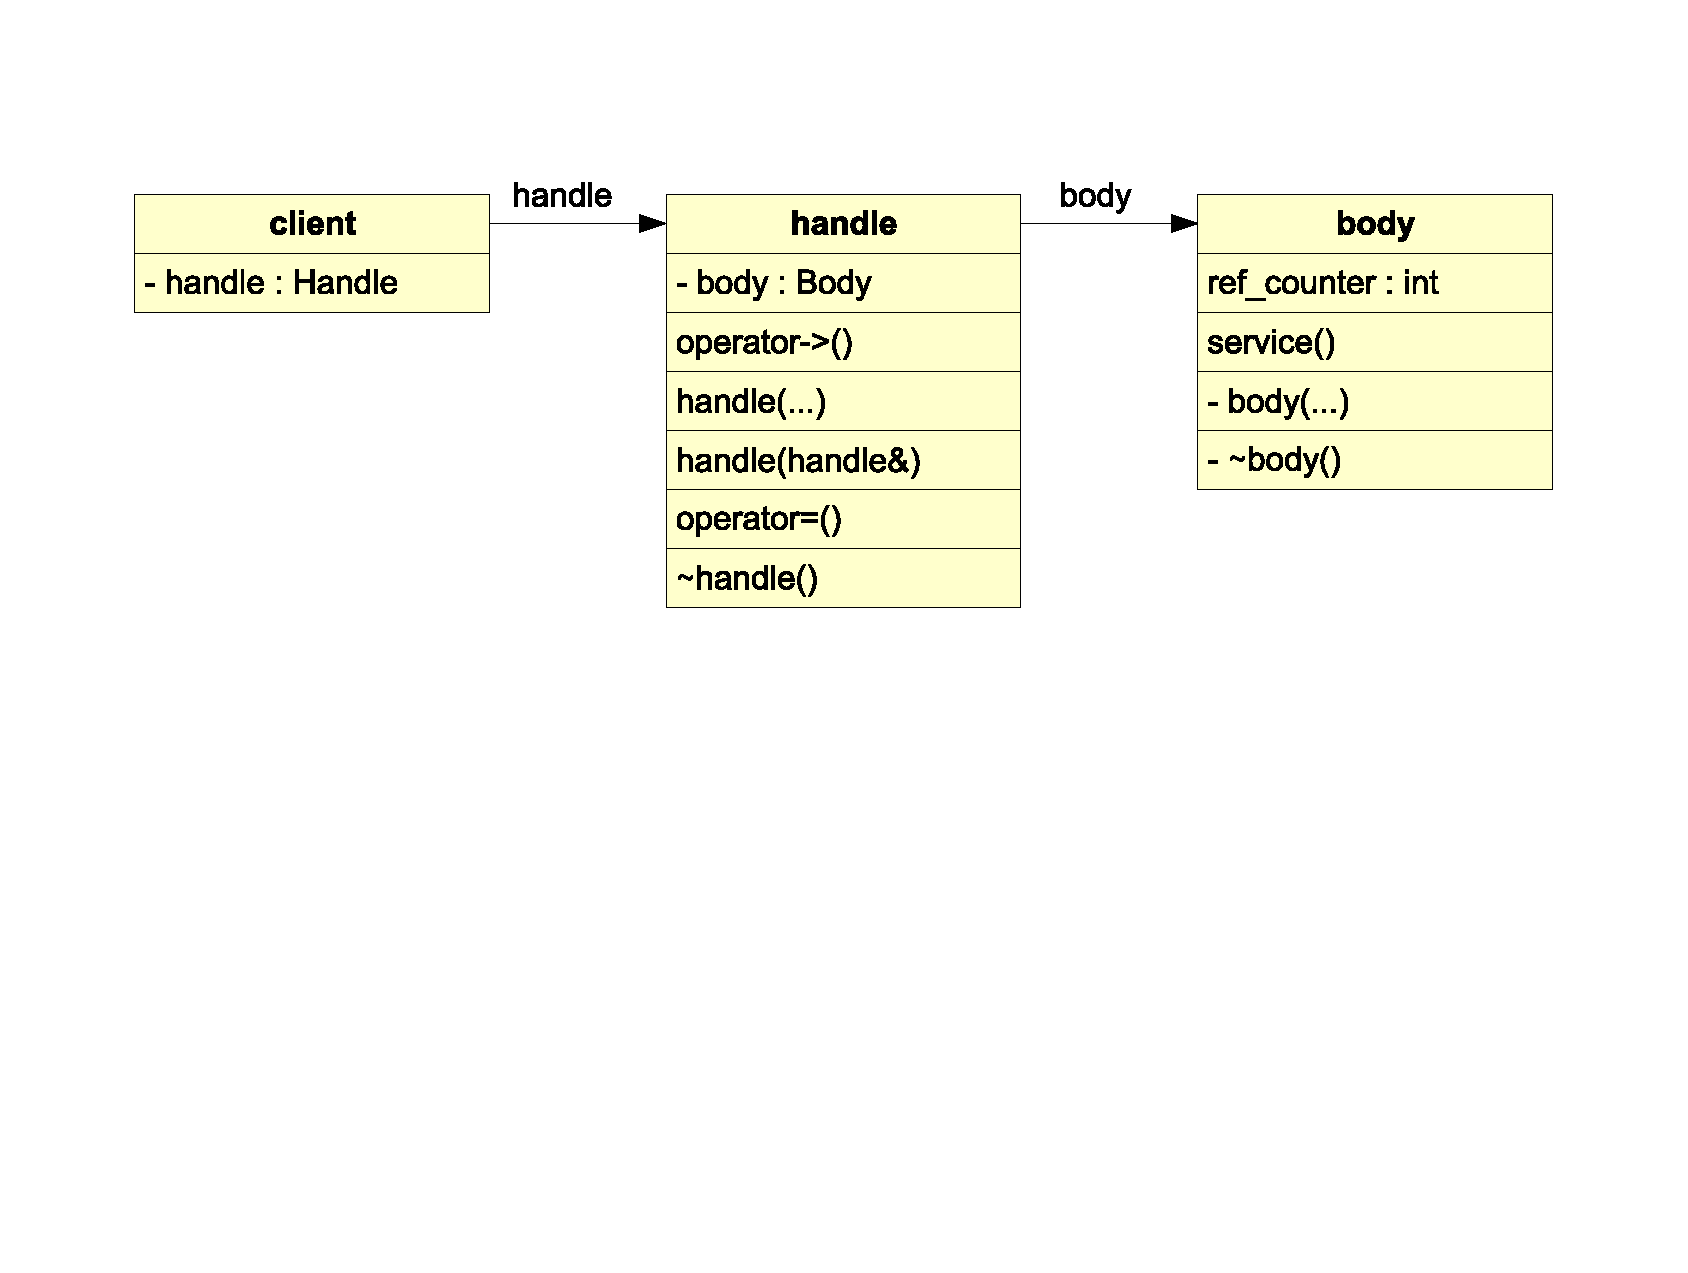
\includegraphics[scale=0.3]{vector/pointer.eps}
        \caption{Counted Pointer Pattern}
        \label{pointer_figure}
    \end{center}
\end{figure}
